\section{Architekturbild \& Buildprozess}
Die Anfragen werden vom Browser über HTTPS an den \textbf{HAProxy}-Loadbalancer gesendet. Dieser verteilt sie an den Docker-Container, in dem \textbf{Tomcat} als Application-Server läuft. Tomcat verarbeitet die Anfragen und greift dabei auf \textbf{Redis} als Warteschlange für Hintergrundaufgaben sowie über \textbf{JDBC} auf die \textbf{MariaDB} zur persistenten Datenspeicherung zu. Links unten ist die Entwicklungsumgebung mit der Verzeichnisstruktur \textit{(bin/, build/, src/, app/, target/ und local/)} dargestellt. Von dort aus wird die Anwendung erstellt (Build) und über den \textbf{Tomcat Manager} im Docker-Container bereitgestellt (Deploy).
\begin{figure}[H]
  \centering
  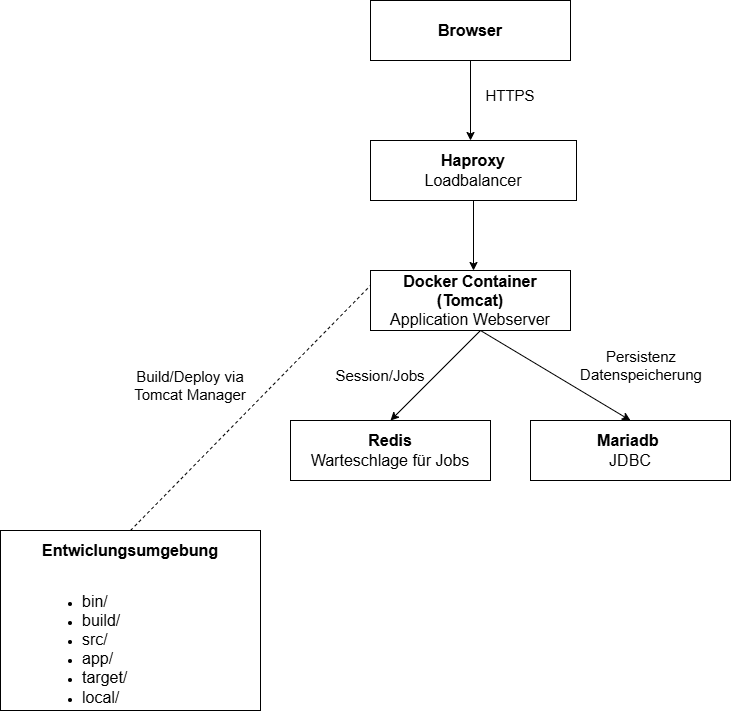
\includegraphics[width=1\linewidth]{src/abbildungen/Architektur.png}
  \caption{Architekturbild}
\end{figure}
    \textbf{Buildprozess:}
   \begin{center}
     \centering
     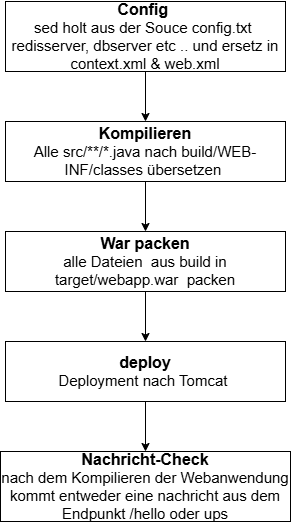
\includegraphics[width=0.9\linewidth]{src/abbildungen/struktur.png}
     \captionof{figure}{build-Prozess}
   \end{center}
